\let\negmedspace\undefined
\let\negthickspace\undefined
\documentclass[journal]{IEEEtran}


\setlength{\headheight}{1cm} % Set the height of the header box
\setlength{\headsep}{0mm}     % Set the distance between the header box and the top of the text
 \usepackage[a4paper,margin=10mm, onecolumn]{geometry}
\usepackage{gvv-book}
\usepackage{gvv}
\usepackage{cite}
\usepackage{amsmath,amssymb,amsfonts,amsthm}
\usepackage{algorithmic}
\usepackage{graphicx}
\usepackage{textcomp}
\usepackage{xcolor}
\usepackage{txfonts}
\usepackage{listings}
\usepackage{enumitem}
\usepackage{mathtools}
\usepackage{gensymb}
\usepackage{comment}
\usepackage[breaklinks=true]{hyperref}
\usepackage{tkz-euclide} 
\usepackage{listings}                                       
\def\inputGnumericTable{}                                
\usepackage[latin1]{inputenc}                                
\usepackage{color}                                            
\usepackage{array}                                            
\usepackage{longtable}                                       
\usepackage{calc}                                             
\usepackage{multirow}                                         
\usepackage{hhline}                                           
\usepackage{ifthen}                                           
\usepackage{lscape}
\usepackage{circuitikz}
\tikzstyle{block} = [rectangle, draw, fill=blue!20, 
    text width=4em, text centered, rounded corners, minimum height=3em]
\tikzstyle{sum} = [draw, fill=blue!10, circle, minimum size=1cm, node distance=1.5cm]
\tikzstyle{input} = [coordinate]
\tikzstyle{output} = [coordinate]

\begin{document}

\bibliographystyle{IEEEtran}
\vspace{3cm}

\title{1.11.13}
\author{AI25BTECH11011-VARUN}
 \maketitle
% \newpage
% \bigskip
{\let\newpage\relax\maketitle}

\renewcommand{\thefigure}{\theenumi}
\renewcommand{\thetable}{\theenumi}
\setlength{\intextsep}{10pt} % Space between text and floats


\numberwithin{equation}{enumi}
\numberwithin{figure}{enumi}
\renewcommand{\thetable}{\theenumi}
\textbf{Question}:\\
If a line makes angles 90$\degree$,135$\degree$,45$\degree$ with the x, y and z axes respectively,find its direction cosines.  \\
\textbf{Solution}:\\
The direction cosines of a vector $\vec{A}$ making $\alpha$, $\beta$ and $\gamma$ angles with x,y and z axes respectively is,

\begin{align}
    \vec{A} = \myvec{\cos{\alpha} \\ \cos{\beta} \\ \cos{\gamma}}
\end{align}

Then, the direction vector is,

\begin{align}
    \vec{A} = \myvec{\cos{90\degree} \\ \cos{135\degree} \\ \cos{45\degree}}  \\
    \vec{A} = \myvec{0 \\ -\frac{1}{\sqrt{2}} \\ \frac{1}{\sqrt{2}}}
\end{align}

\begin{figure}[H]
    \centering
    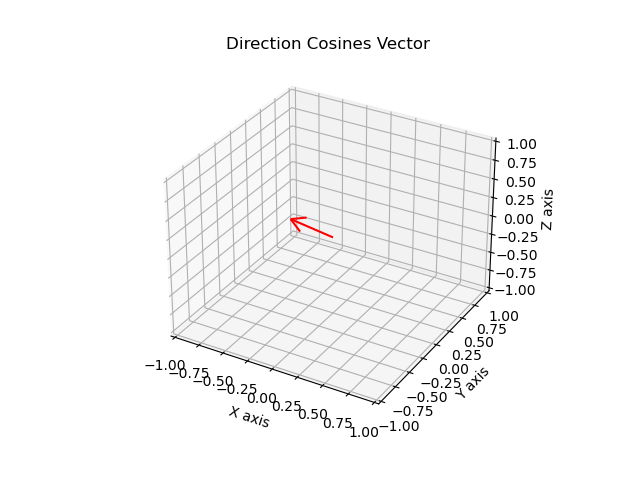
\includegraphics[width=0.8\textwidth]{figs/Fig 1.png}
    \caption{}
    \label{fig:Parallelogram}
\end{figure}

\end{document}
